\documentclass[11pt]{beamer}
\usepackage[utf8]{inputenc}
\usetheme{Boadilla}
\setbeamertemplate{navigation symbols}{}
\usepackage{lmodern}
\usepackage[T2A]{fontenc}
\usepackage{cmbright}
\usepackage[russian, english]{babel}
%\usetheme{Darmstadt}

\usetheme{Boadilla}
\setbeamertemplate{navigation symbols}{}

\usepackage{amsmath}
\usepackage{amsfonts}
\usepackage{bm}
\usepackage{graphicx}
\usepackage{xcolor}
\usepackage{wrapfig}
% Использовать полужирное начертание для векторов
\let\vec=\mathbf

\DeclareMathOperator{\mathspan}{span}
\DeclareMathOperator{\mathdim}{dim}
\DeclareMathOperator{\rank}{rank}
\DeclareMathOperator{\diag}{diag}
\begin{document}
	\author{Е. Ларин, Ф. Ежов, И. Кононыхин }
	\title[Neural Nets]{Neural Nets (NN), с элементами Deep Learning}
	%\subtitle{}
	%\logo{}
	\institute[]{Санкт-Петербургский государственный университет 
		
		Прикладная математика и информатика
		
		Вычислительная стохастика и статистические модели
	}
	\date{}
	\subject{Семинар по статистическому и машинному обучению}
	\setbeamercovered{transparent}
	\setbeamertemplate{navigation symbols}{}
	
	\begin{frame}[plain]
		\maketitle 
	\end{frame}
	
	\begin{frame}
		\frametitle{Математическая модель нейрона}
		
		\begin{figure}[h]
			\begin{minipage}[h]{0.49\linewidth}
				\center{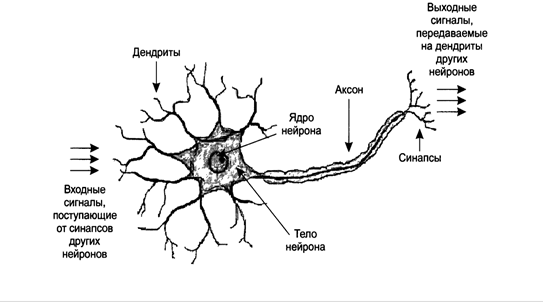
\includegraphics[width=1.2\linewidth]{../Report/imgs/bio_neuron}}
			\end{minipage}
			\hfill
			\begin{minipage}[h]{0.49\linewidth}
				\center{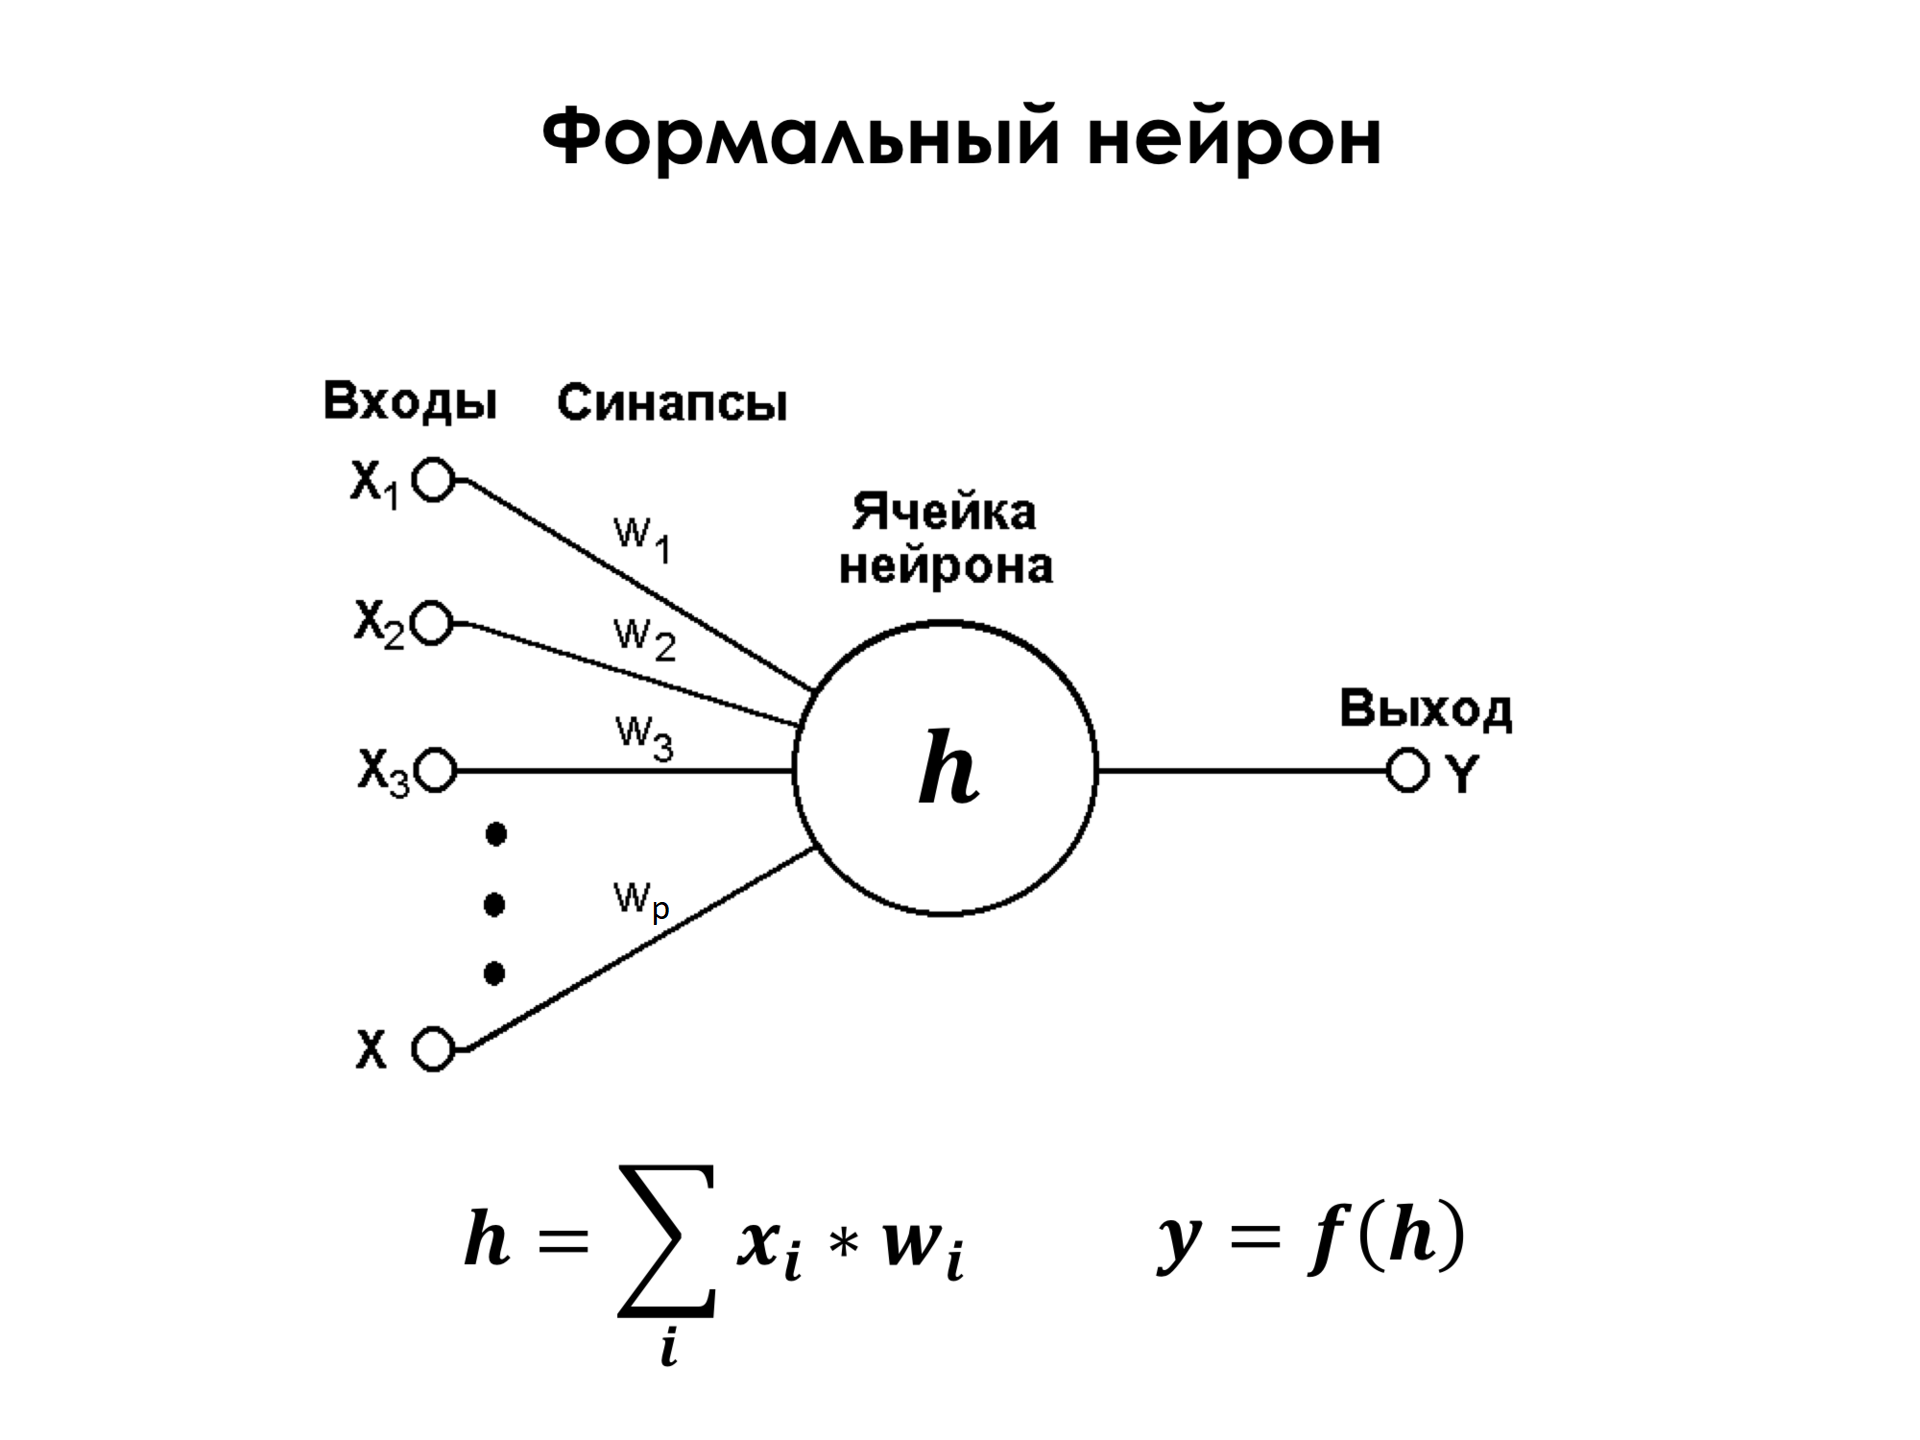
\includegraphics[width=1.2\linewidth]{../Report/imgs/math_neuron}}
			\end{minipage}
		\end{figure}
		
	\end{frame}

	\begin{frame}
		\frametitle{Перцептрон}
		
		\begin{wrapfigure}{L}{0.4\linewidth} %this figure will be at the right
			\centering
			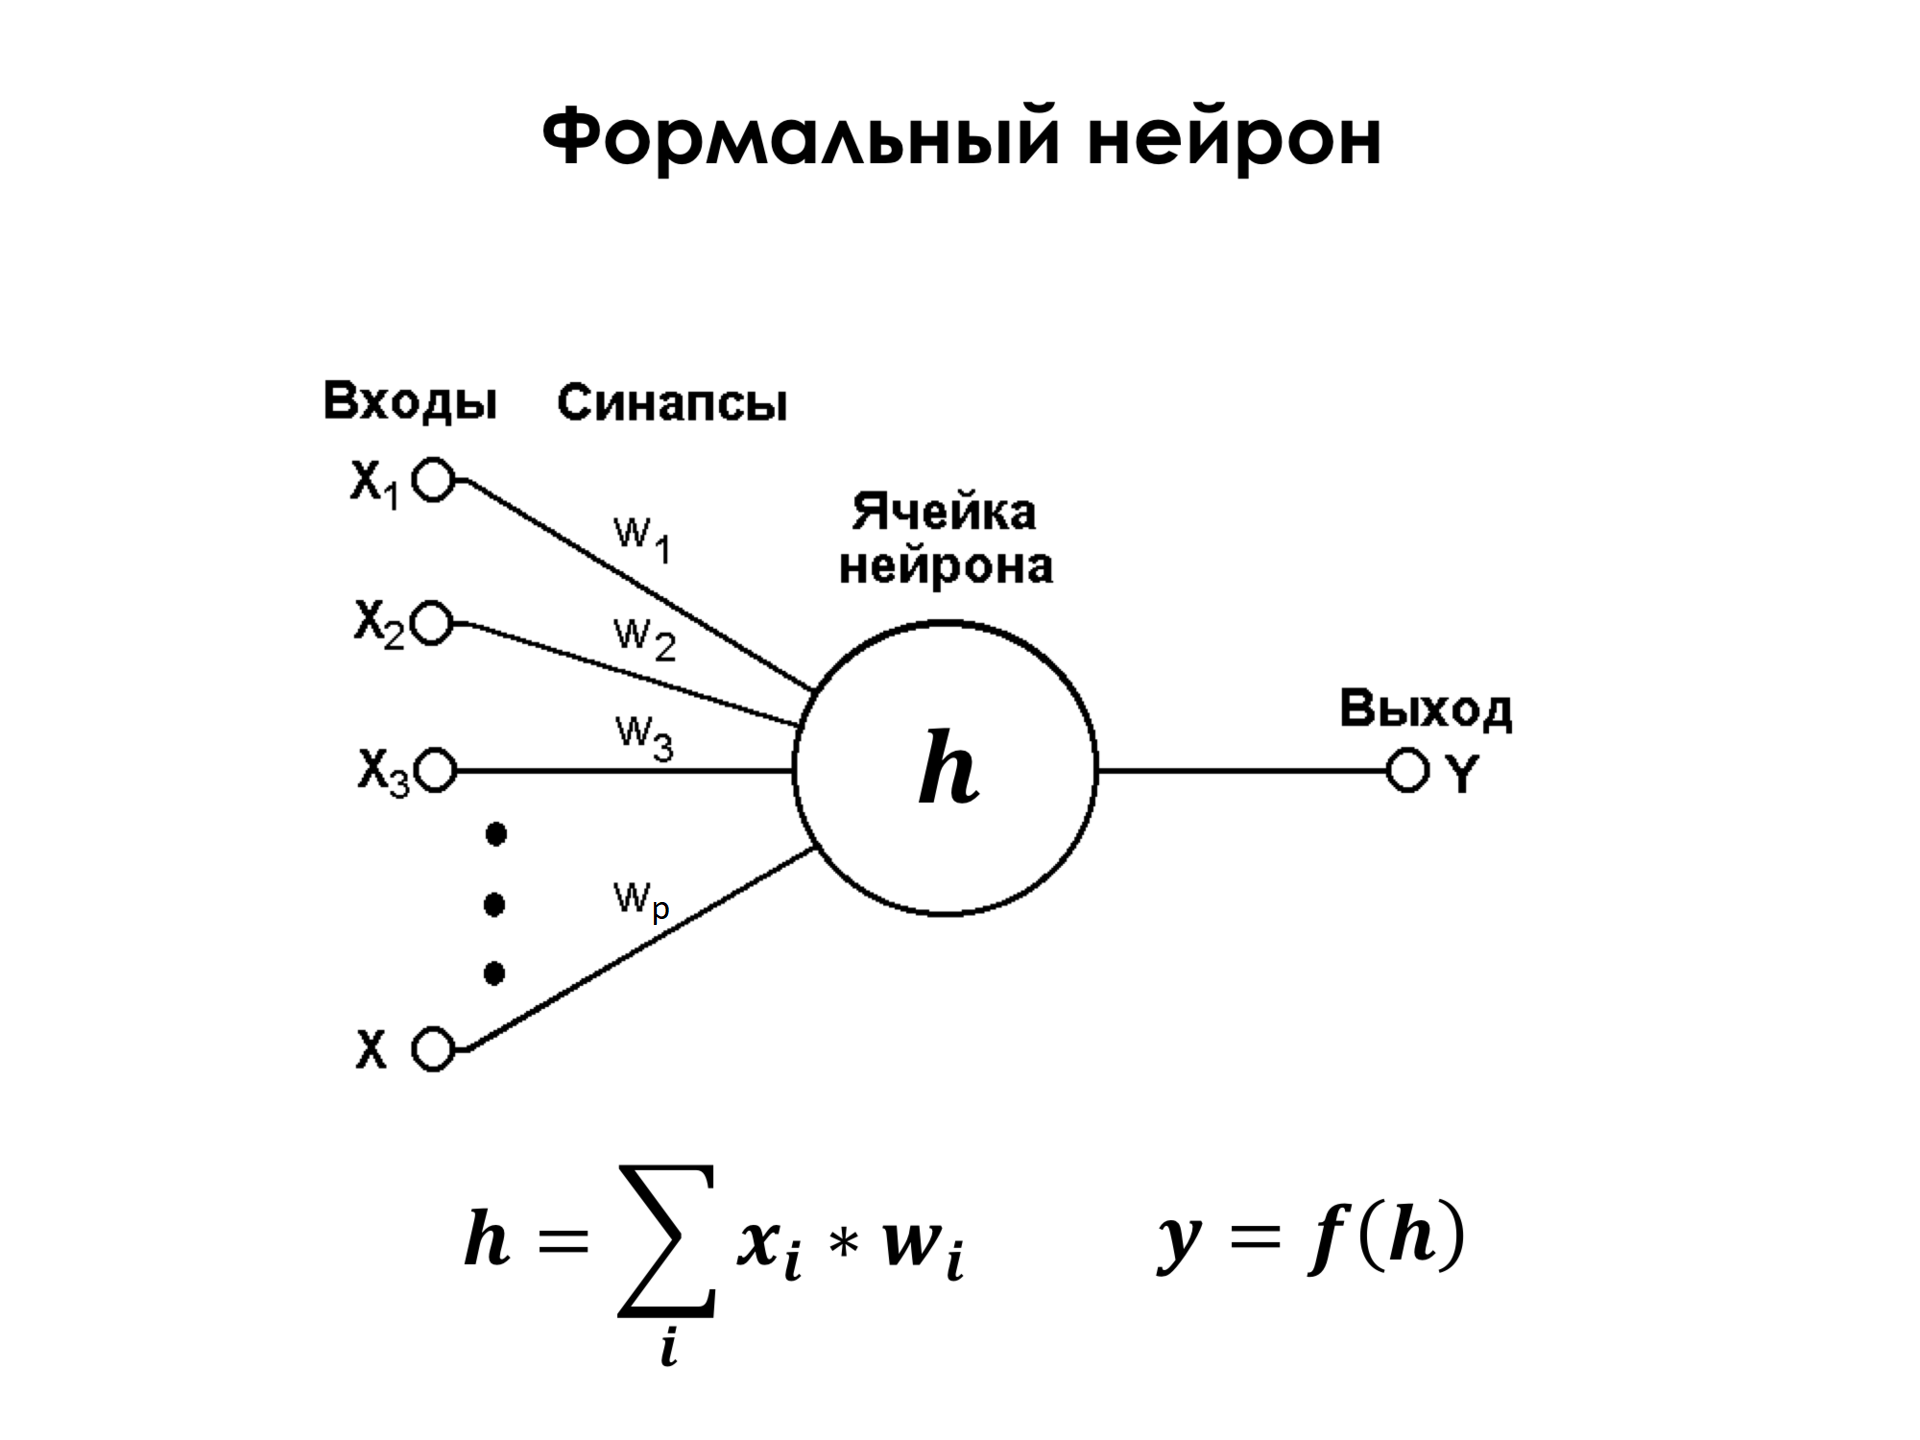
\includegraphics[width=1.2\linewidth]{../Report/imgs/math_neuron}
		\end{wrapfigure}
	
		Перцептрон(perceptron) --- одна из простейших архитектур ANN, придуманная Фрэнком Розенблаттом в 1957 году. \\
		
		
		\begin{itemize}
		\item $p$ --- количество признаков
		\item $\{ x_1, \cdots, x_p \}$ --- индивид. 
		\item $\{ w_1, \cdots, w_p \}$ --- веса нейрона. 
		\item \begin{equation*} 
			f(h) =  \begin{cases}
					0 & h < 0 \\
					1 & h \geqslant 0
					\end{cases}
		\end{equation*}
		--- функция активации. 
		\item $y$ --- выход сети.
		\end{itemize}
		
	
		
	\end{frame}

	%\begin{frame}
	%	\frametitle{Перцептрон: Обучение}
		
	%	Образцы $x_i$ подаются по одному.
		
	%	{\color{blue}Изменение весов перцептерона:} $w^{next}_{i,j} = w_{i,j} + \eta (y_i - \hat{y_i}) x_i$
		
	%	\begin{itemize}
	%		\item $w_{i,j}$ --- вес связи между $i$-ым входным нейроном и $j$-ым выходным нейроном.
	%		\item $x_i$ --- $i$-ое входное значение текущего образца.
	%		\item $\hat{y_i}$ --- выход $j$-го выходного нейрона для текущего обучающего образца.
	%		\item $y_i$ --- целевой выход $j$-го выходного нейрона для текущего обучающего образца.
	%		\item $\eta$ --- скорость обучения.
	%	\end{itemize}
			
		
	%\end{frame}
	

	\begin{frame}
		\frametitle{Перцептрон: Проблемы}
	
		
		Перцептрон может решать только линейно разделимые задачи.
		
		\begin{block}{Проблема}
			Перцептрон не способен решить некоторые тривиальные задачи, например задачу классификации на основе исключающего "ИЛИ" (Exclusive OR - XOR). 
		\end{block}
		
		
	\end{frame}

	\begin{frame}
		\frametitle{MultiLayer Perceptron (MLP)}
		
		Каждый слой кроме выходного включает нейрон смещения и полностью связан со следующим слоем.
		
		\begin{figure}[h]
			\center{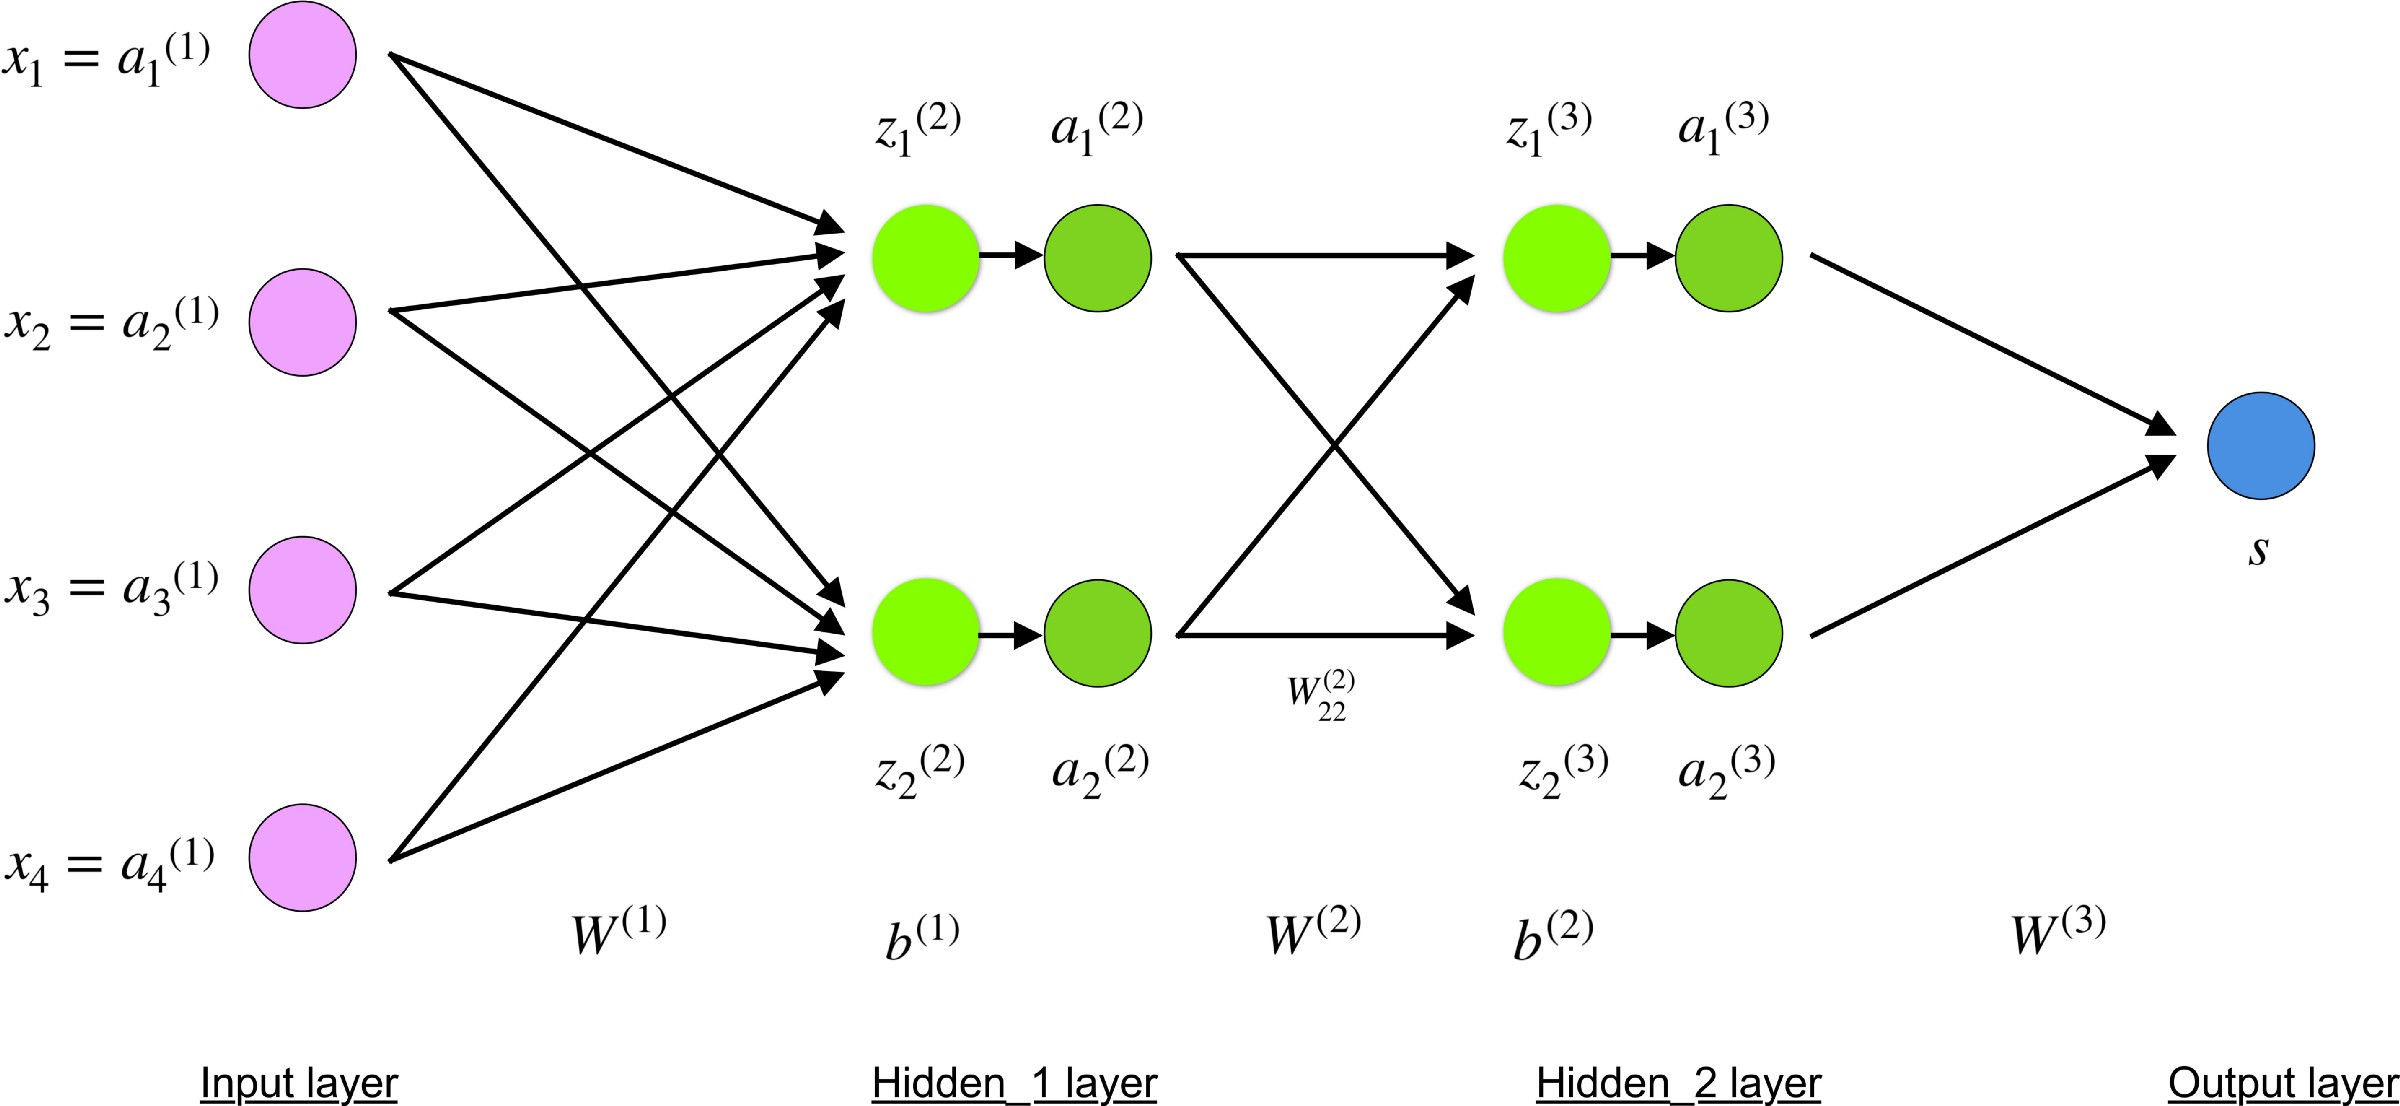
\includegraphics[width=0.7\linewidth]{../Report/imgs/MLP}}
		\end{figure}
		
		
	\end{frame}


	\begin{frame}
		\frametitle{MultiLayer Perceptron (MLP): Теорема Цыбенко}
		
		Функция $\sigma(z)$ --- сигмоида, если $\lim\limits_{z 	\rightarrow -\infty}\sigma(z) = 0$ и $\lim\limits_{z 	\rightarrow +\infty}\sigma(z) = 1$.
		
		\begin{block}{Теорема Цыбенко}
			Если функция активации $\sigma(z)$ --- непрерывная сигмоида, то для любой непрерывной на $[0, 1]^p$ функции $f(x)$ существуют такие значение параметров $w_h \in \mathbb{R}^p, w_0 \in \mathbb{R}, \alpha_h \in \mathbb{R} $, что двухслойная сеть 
			$$ a(x) = \sum\limits_{h=1}^H \alpha_h \sigma( \langle x, w_h \rangle + w_0) $$
			
			равномерно приближает $f(x)$ с любой точность $\varepsilon$:
			$$ |a(x) - f(x)| < \varepsilon, \text{для всех} x \in [0, 1]^p $$
		\end{block}
		
		
	\end{frame}

		\begin{frame}
		\frametitle{MultiLayer Perceptron (MLP): Функции представимые нейросетью}

		\begin{itemize}
			\item Двухслойная сеть в $\mathbb{R}^p$ позволяет отделить произвольный выпуклый многогранник.
			\item Трехслойная сеть в $\mathbb{R}^p$ позволяет отделить произвольную многогранную область, не обязательно выпуклую, и даже не обязательно связную.
			\item С помощью линейных операций и одной нелинейной функции активации можно приблизить любую непрерывную функцию с любой желаемой точностью.
		\end{itemize}
		
		
		
	\end{frame}

	\begin{frame}
		\frametitle{Обучение MLP}
		
		\begin{figure}[h]
			\center{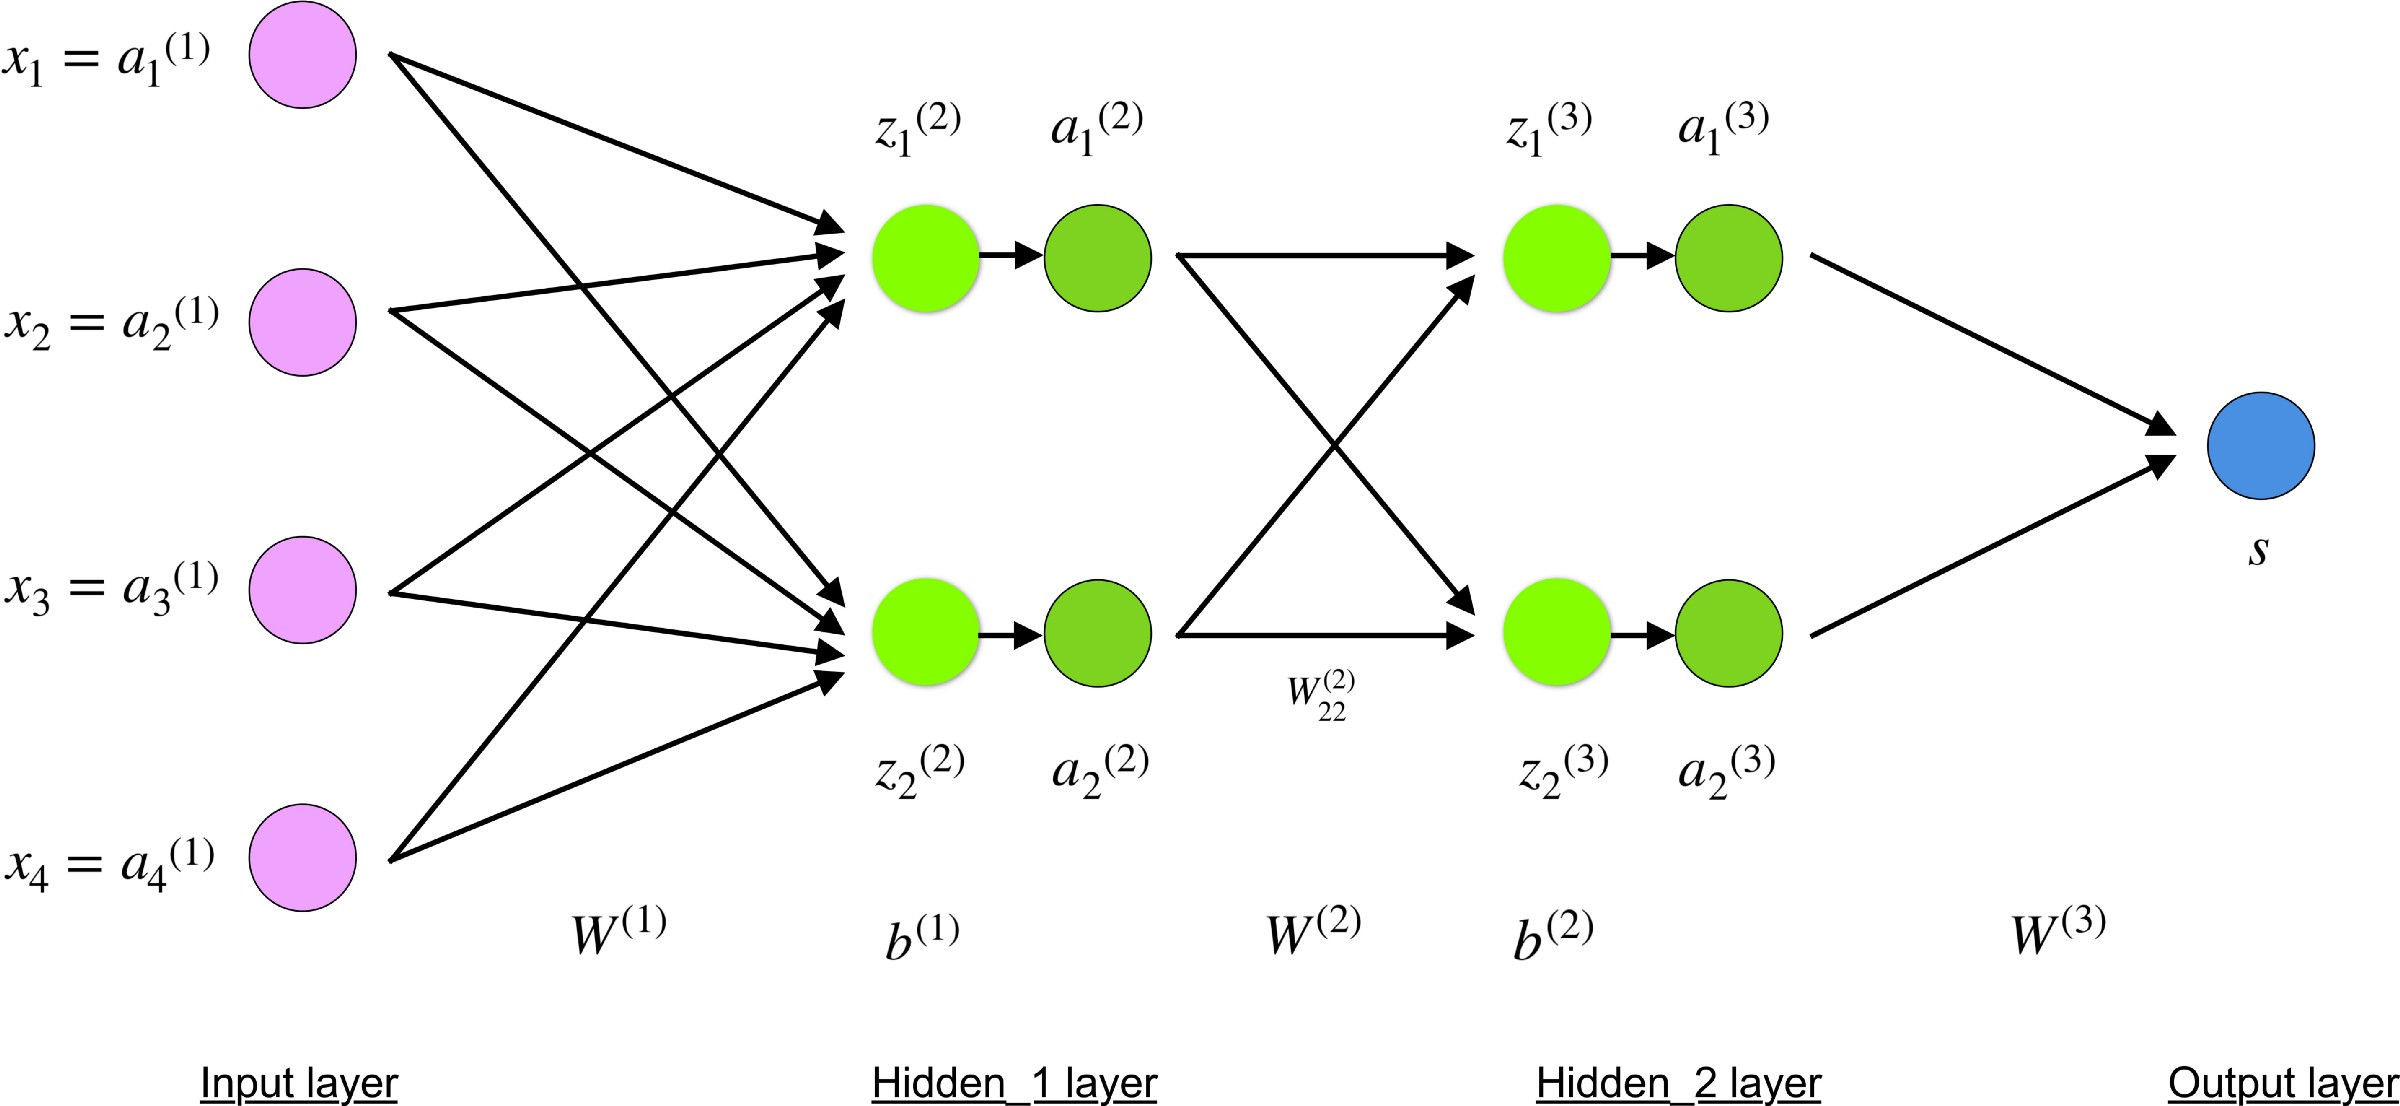
\includegraphics[width=0.7\linewidth]{../Report/imgs/MLP}}
		\end{figure}
		
		Минимизация средних потерь на обучающей выборке:
		
		$$ Q(w) := \dfrac{1}{n} \sum\limits_{i=1}^{n} \mathcal{C}_i(w) \rightarrow \min\limits_w  $$
	%	\begin{block}{}
			%Многократно корректирует веса соединений в сети таким образом, чтобы минимизировать меру разницы %между фактическим выходным вектором сети и желаемым выходным вектором.
	%	\end{block}
		
		$\mathcal{C}$ --- любая дифференцируемая функция потерь.
		
	\end{frame}

	\begin{frame}
		\frametitle{Алгоритм SG}
		
		
		{\color{blue}Задача минимизации:} $ Q(w) := \dfrac{1}{n} \sum\limits_{i=1}^{n} \mathcal{C}_i(w) \rightarrow \min\limits_w  $
		
		{\color{blue} Вход:} выборка $X^n$; <<скорость>> обучение $\epsilon$; параметр $\lambda$;
		
		{\color{blue} Выход:} оптимизированные значение весов $w$.
		
		\begin{enumerate}
			\item инициализация весов $w$ и текущую оценку $Q(w)$
			\item {\color{blue} повторять}
			\item выбрать объект $x_i$ из $X^n$;
			\item вычислить потерю $\mathcal{C}_i := \mathcal{C}_i(w)$
			\item градиентный шаг: $w := w - \epsilon \mathcal{C}_i^{'}(w)$
			\item оценить значение функционала: $Q := (1-\lambda)Q + \lambda \mathcal{C}_i$
			\item {\color{blue} пока} значение $Q$ и/или весов $w$ не стабилизируются
		\end{enumerate}	
		
		
	\end{frame}

	\begin{frame}
		\frametitle{Обучение MLP: forward-propagation }
		
		\begin{figure}[h]
			\center{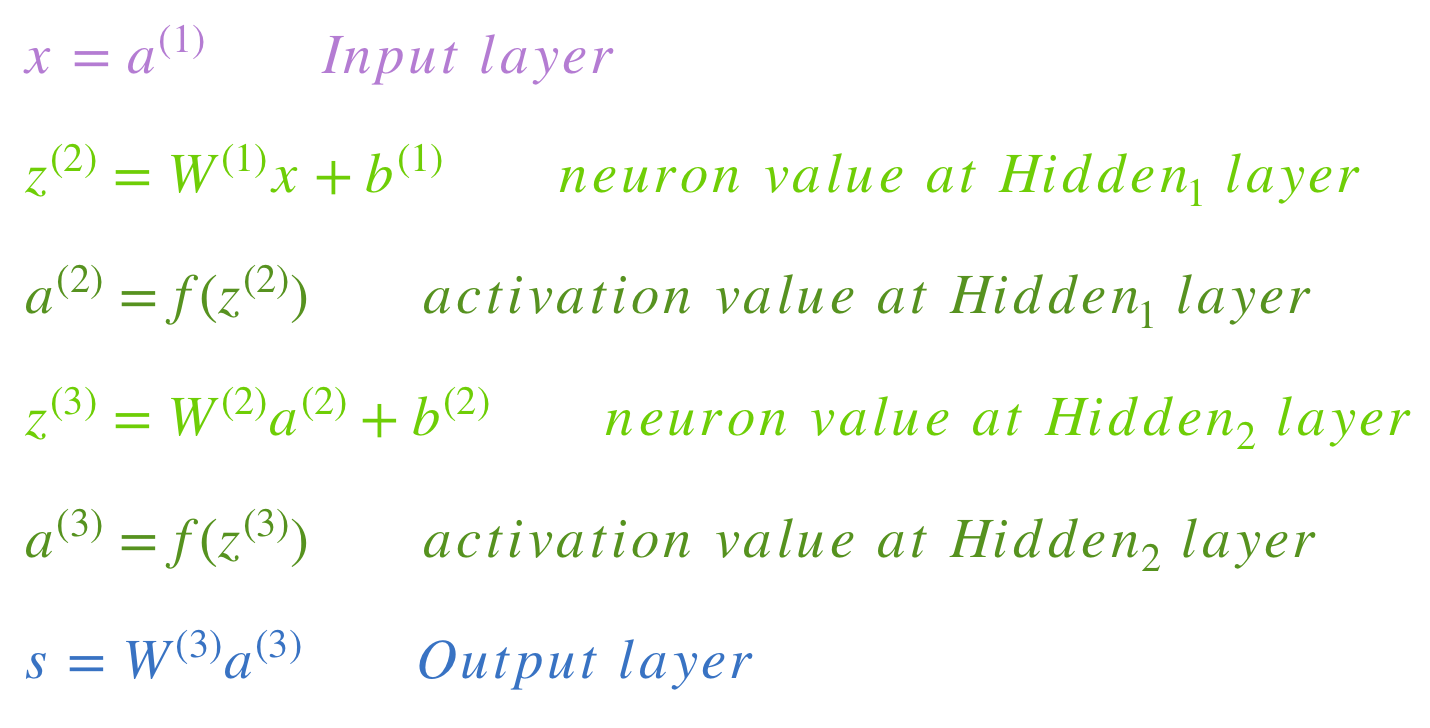
\includegraphics[width=0.7\linewidth]{../Report/imgs/forwardprop}}
		\end{figure}
	
		\begin{figure}[h]
			\center{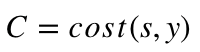
\includegraphics[width=0.2\linewidth]{../Report/imgs/cost_function}}
		\end{figure}
	
		$s$ --- полученная оценка с помощью нейронной сети. $y$ --- правильный ответ. $\mathcal{C}$ --- значение ошибки между $s$ и $y$ по какой-нибудь метрики (например MSE).
		
	\end{frame}

	\begin{frame}
		\frametitle{Обучение MLP: back-propagation }
		
		\begin{figure}[h]
			\center{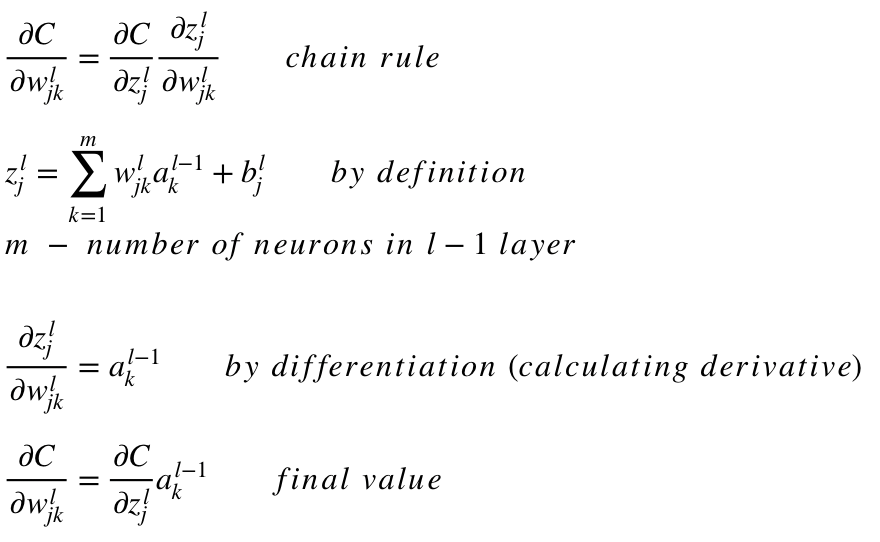
\includegraphics[width=0.7\linewidth]{../Report/imgs/chain-rule}}
		\end{figure}
		
	\end{frame}

	\begin{frame}
		\frametitle{Обучение MLP: процесс изменения весов }
		
		\begin{figure}[h]
			\center{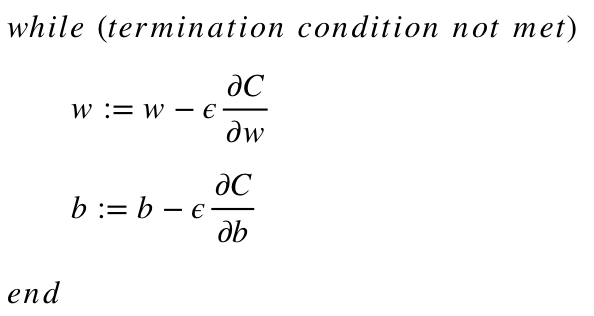
\includegraphics[width=0.7\linewidth]{../Report/imgs/weigh_change_process}}
		\end{figure}
		
	\end{frame}

	
	\begin{frame}
		\frametitle{back-propagation algorithm: в итоге}
		{\color{blue} Преимущества:} 
			\begin{itemize}
				\item быстрое вычисление градиента
				\item обобщение на любые функции активации, функции потерь и количество слоев
				\item возможность потокового обучения
				%\item сублинейное обучение на сверхбольших выборках (когда части объектов $x_i$ уже достаточно для обучения)
				\item возможность распараллеливания
			\end{itemize}
		
		{\color{blue} Недостатки:} 
		\begin{itemize}
			\item медленная сходимость
			\item застревания в локальных экстремумах
			\item проблема переобучения
		\end{itemize}
	
	
	\end{frame}

	\begin{frame}
		\frametitle{Методы решения задачи минимизации}
		
		\begin{itemize}
			\item Stochastic Gradient (SG)
			\item Метод накопления импульса (Momentum)
			\item NAG (Nesterov's accelerated gradient)
			\item RMSProp (running mean square)
			\item AdaDelta (adaptive learning rate)
			\item Adam (adaptive momentum)
			\item Nadam (Nesterov-accelerated adaptive momentume)
		\end{itemize}
	
	\end{frame}
	
	
	\begin{frame}
		\frametitle{Функции активации}
		
		Функции активации добавляют в модель нелинейность.
		
		\begin{figure}[h]
			\center{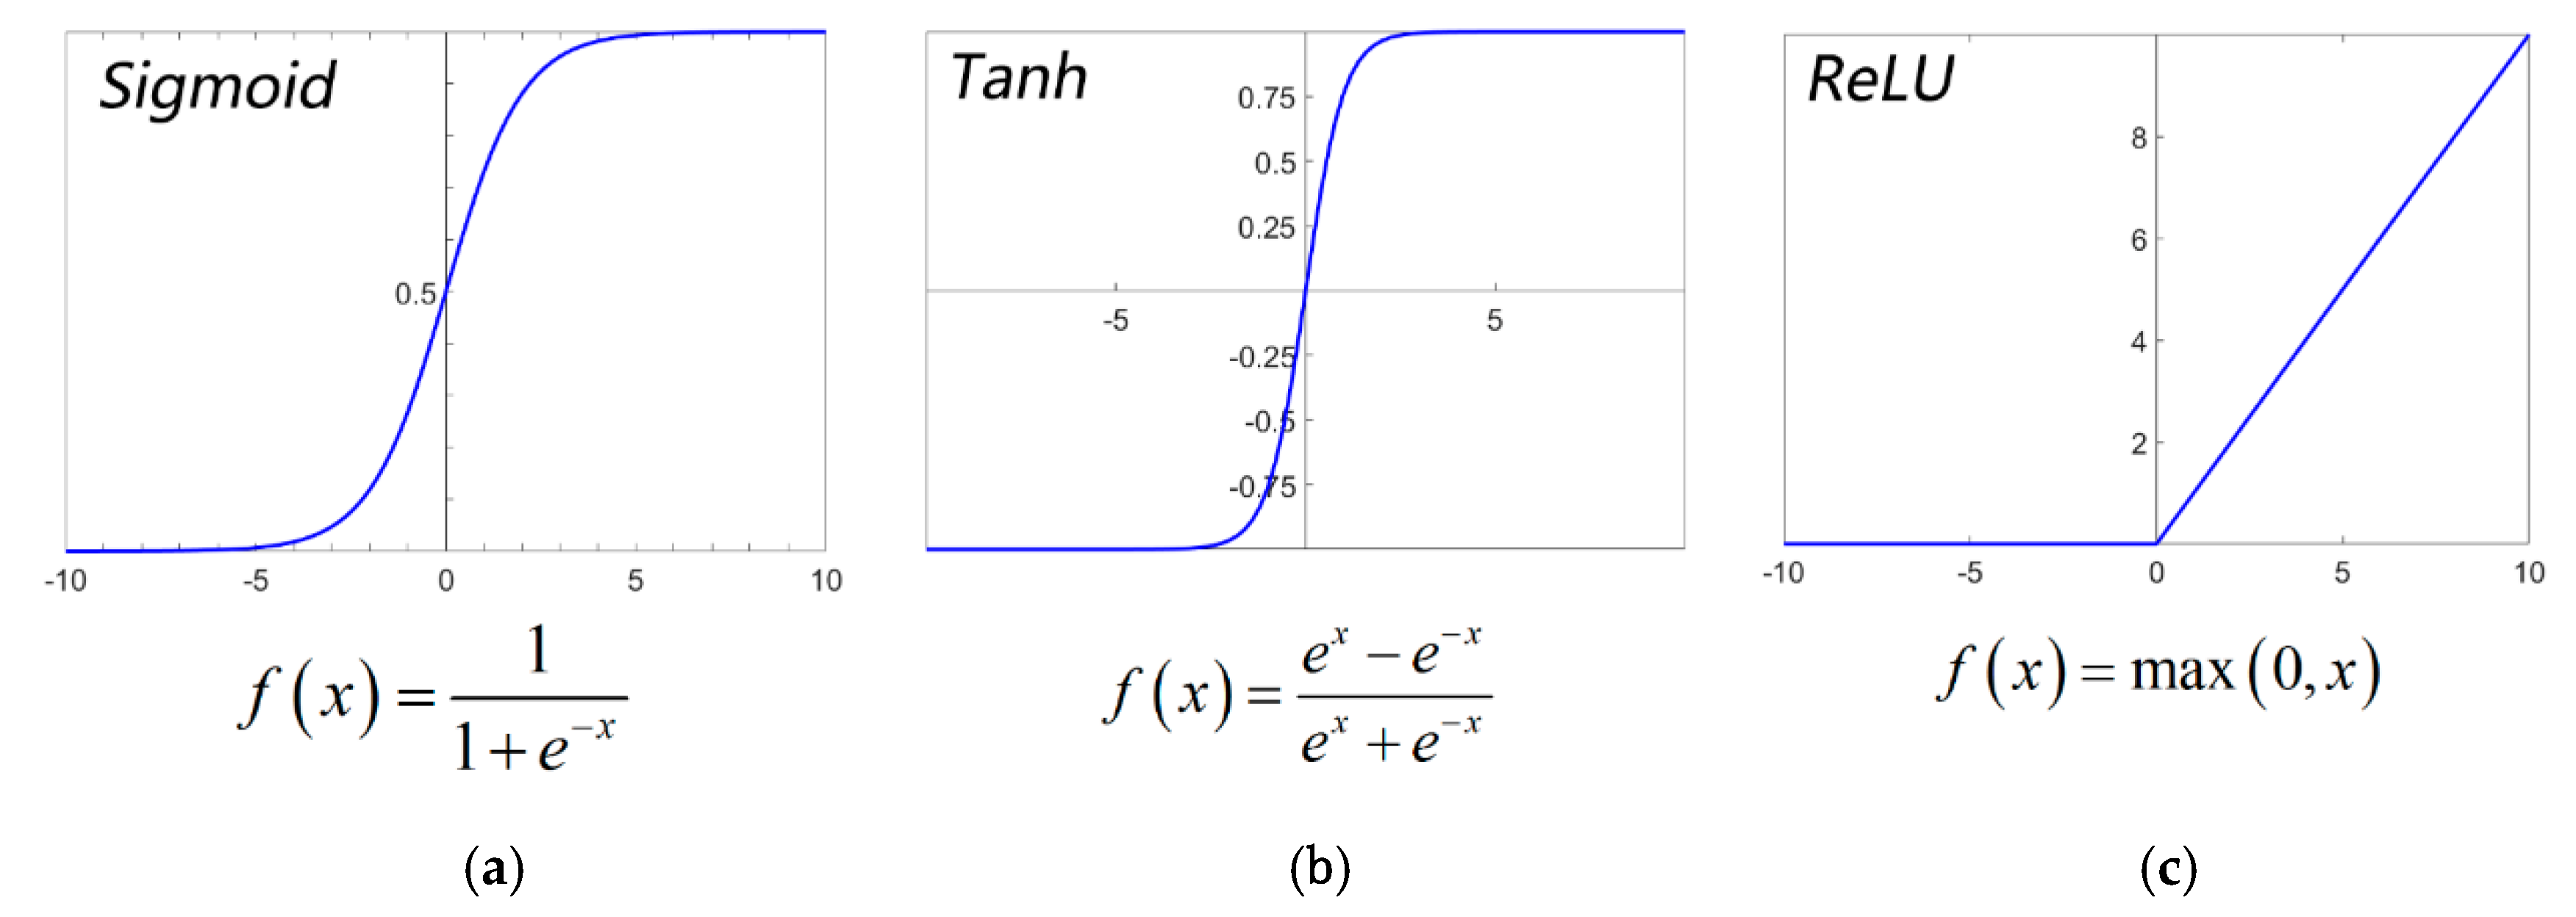
\includegraphics[width=1\linewidth]{../Report/imgs/afuns}}
		\end{figure}
		
	\end{frame}
	
	\begin{frame}
		\frametitle{Recurrent neural network(RNN)}
		
		$x_t$ --- входной вектор в момент времени $t$\\
		$s_t$ --- вектор скрытого слоя в момент времени $t$\\
		$y_t$ --- выходной вектор (в некоторых случаях $y_t \equiv s_t$)
		
		\begin{figure}[h]
			\center{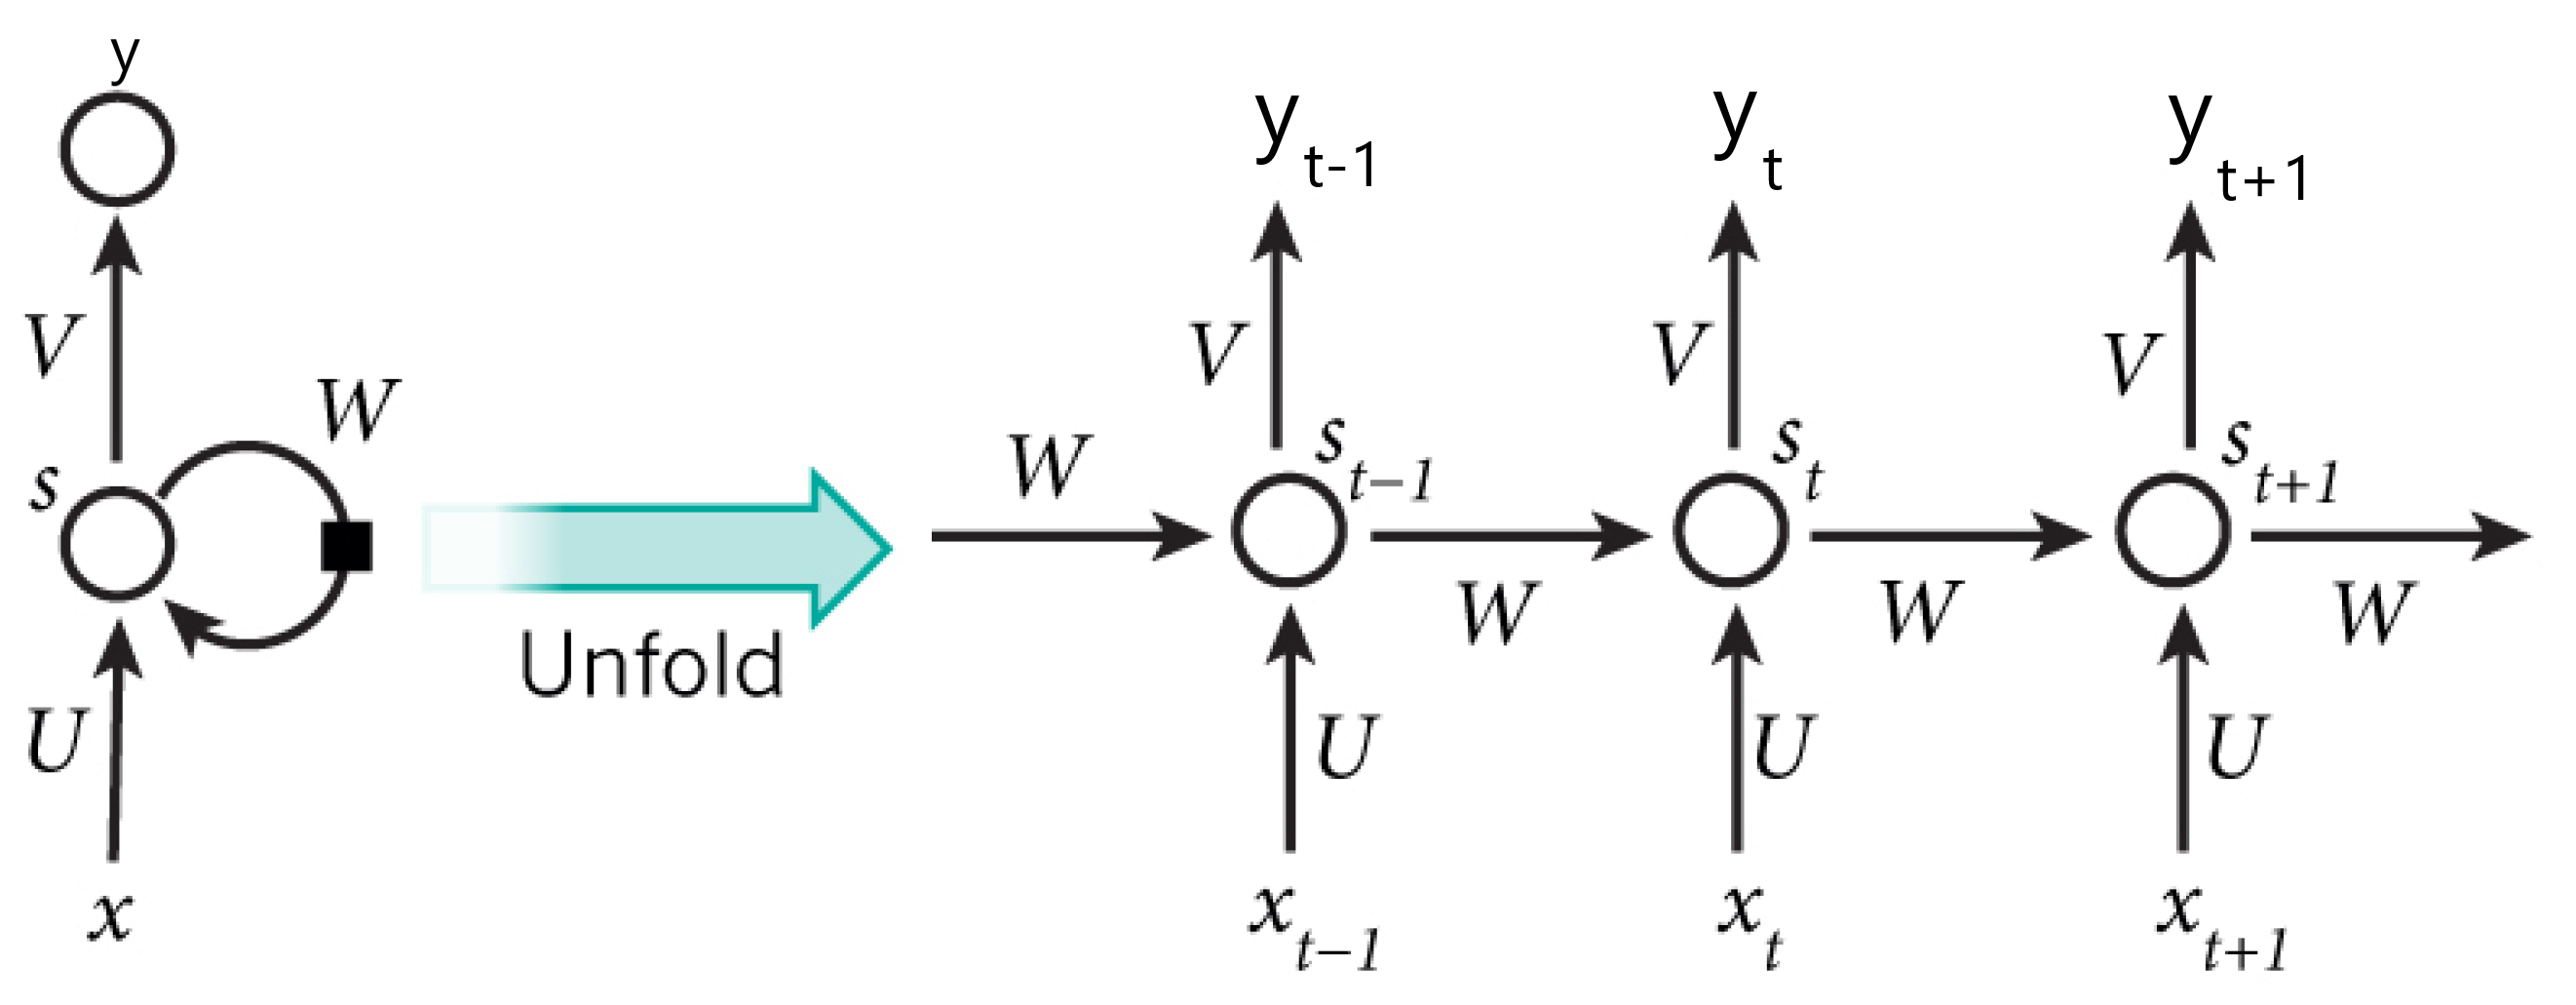
\includegraphics[width=0.5\linewidth]{../Report/imgs/rnn}}
		\end{figure}
	
		Задача:
		$$ \sum\limits_{t=0}^{T}\mathcal{C}_t(U, V, W) \rightarrow \min\limits_{U, V, W}$$
		
		$\mathcal{C}_t(U, V, W) = \mathcal{C}(y_t(U, V, W))$ --- потеря от предсказания $y_t$.
	
	\end{frame}
	
	\begin{frame}
		\frametitle{Обучение RNN}
		Back-propagation Through Time (BPTT)
		
		$$ \dfrac{\partial\mathcal{C}_t}{\partial W} = \dfrac{\partial\mathcal{C}_t}{\partial y_t} \dfrac{\partial y_t}{\partial s_t} \sum\limits_{k=0}^{t} \bigg(  \prod\limits_{i = k+1}^{t}  \dfrac{\partial s_i}{\partial s_{i-1}} \bigg)  \dfrac{\partial h_k}{\partial W}$$
		
		\begin{figure}[h]
			\center{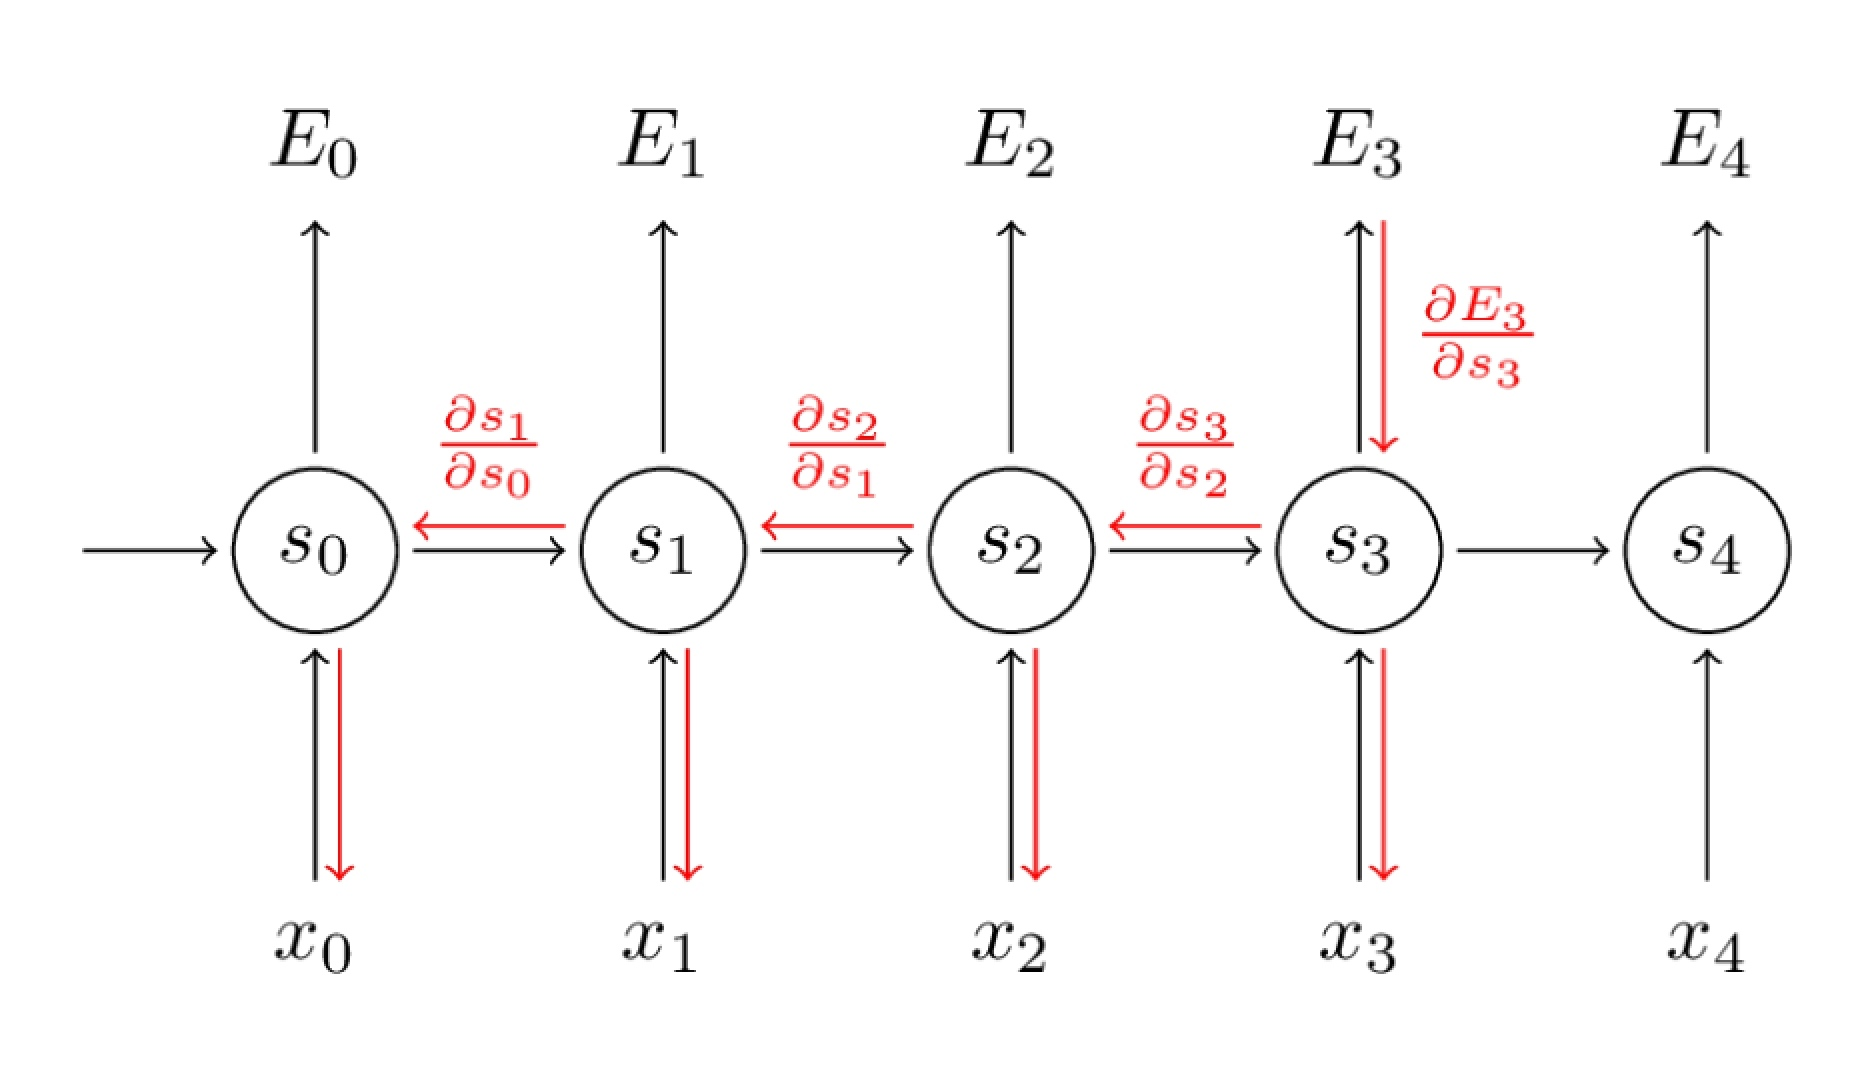
\includegraphics[width=0.5\linewidth]{../Report/imgs/bptt}}
		\end{figure}
		
	\end{frame}

	\begin{frame}
		\frametitle{Где используется RNN?}
		
		\begin{itemize}
			\item Прогнозирование временных рядов
			\item Управление технологическими процессами
			\item Классификация текстов или их фрагментов
			\item Анализ тональности документа / предложений / слов
			\item Машинный перевод
			\item Распознавание речи
			\item Синтез речи
			\item Синтез ответов на вопросы, разговорный интеллект
			\item Генерация подписей к изображениям
			\item Генерация рукописного текста
			\item Интерпретация генома и другие задачи биоинформатики
		\end{itemize}
		
	\end{frame}
	
	\begin{frame}
		\frametitle{Long short-term memory (LSTM)}
		
		{\color{blue} Мотивация LSTM:} сеть должна долго помнить контекст, какой именно --- сеть должна выучить сама.\\
		Вводится $C_t$ --- вектор состояния сети в момент $t$.
		
		\begin{figure}[h]
			\center{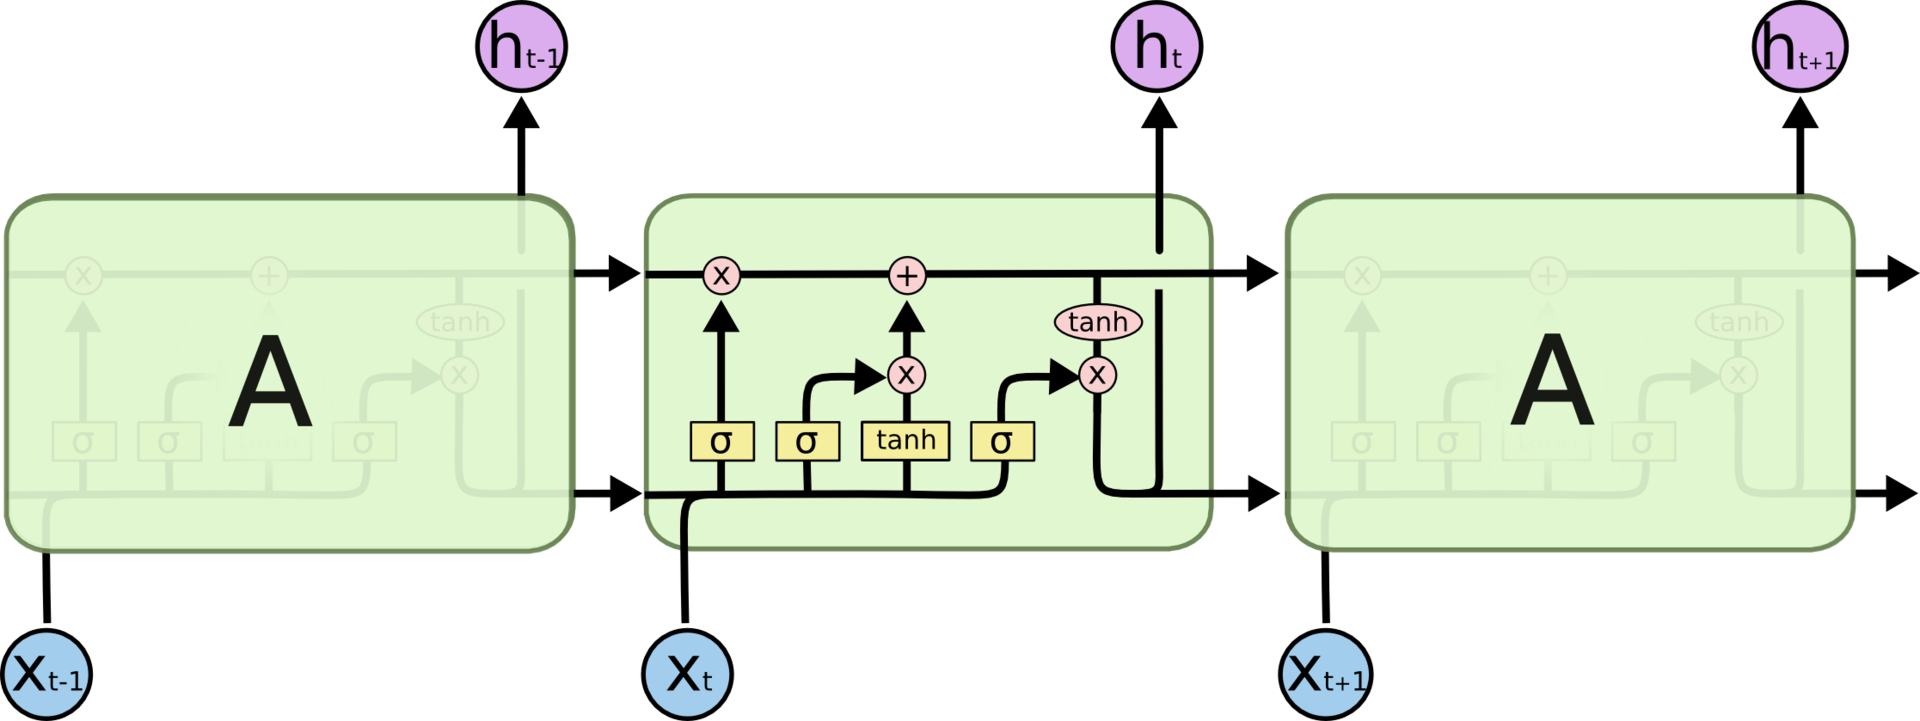
\includegraphics[width=0.8\linewidth]{../Report/imgs/lstm}}
		\end{figure}
	
		\begin{figure}[h]
			\center{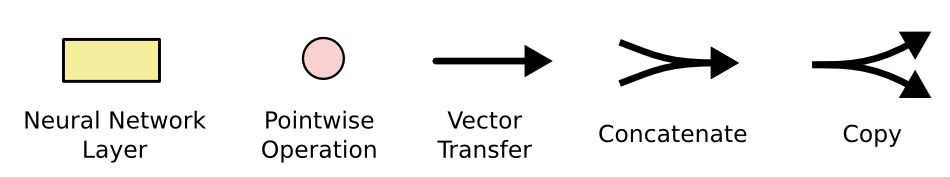
\includegraphics[width=0.6\linewidth]{../Report/imgs/lstm_operations}}
		\end{figure}
		
	\end{frame}

	\begin{frame}
		\frametitle{Объясняя LSTM (часть 1)}
		
		\begin{figure}[h]
			\center{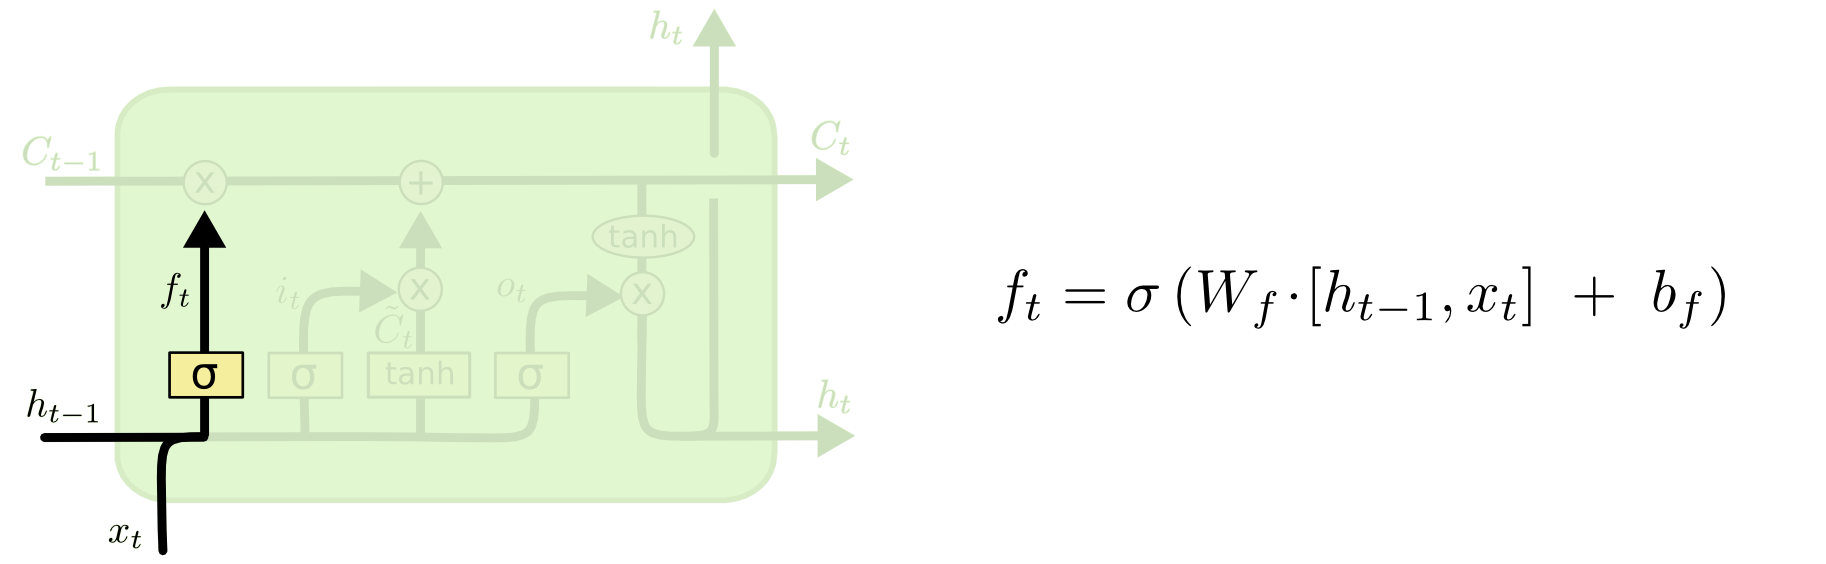
\includegraphics[width=0.8\linewidth]{../Report/imgs/lstm_explanation_step1}}
		\end{figure}
	
		\begin{figure}[h]
			\center{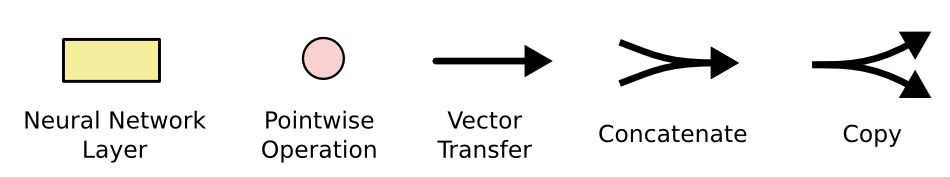
\includegraphics[width=0.6\linewidth]{../Report/imgs/lstm_operations}}
		\end{figure}
	\end{frame}

	\begin{frame}
		\frametitle{Объясняя LSTM (часть 2)}
		
		\begin{figure}[h]
			\center{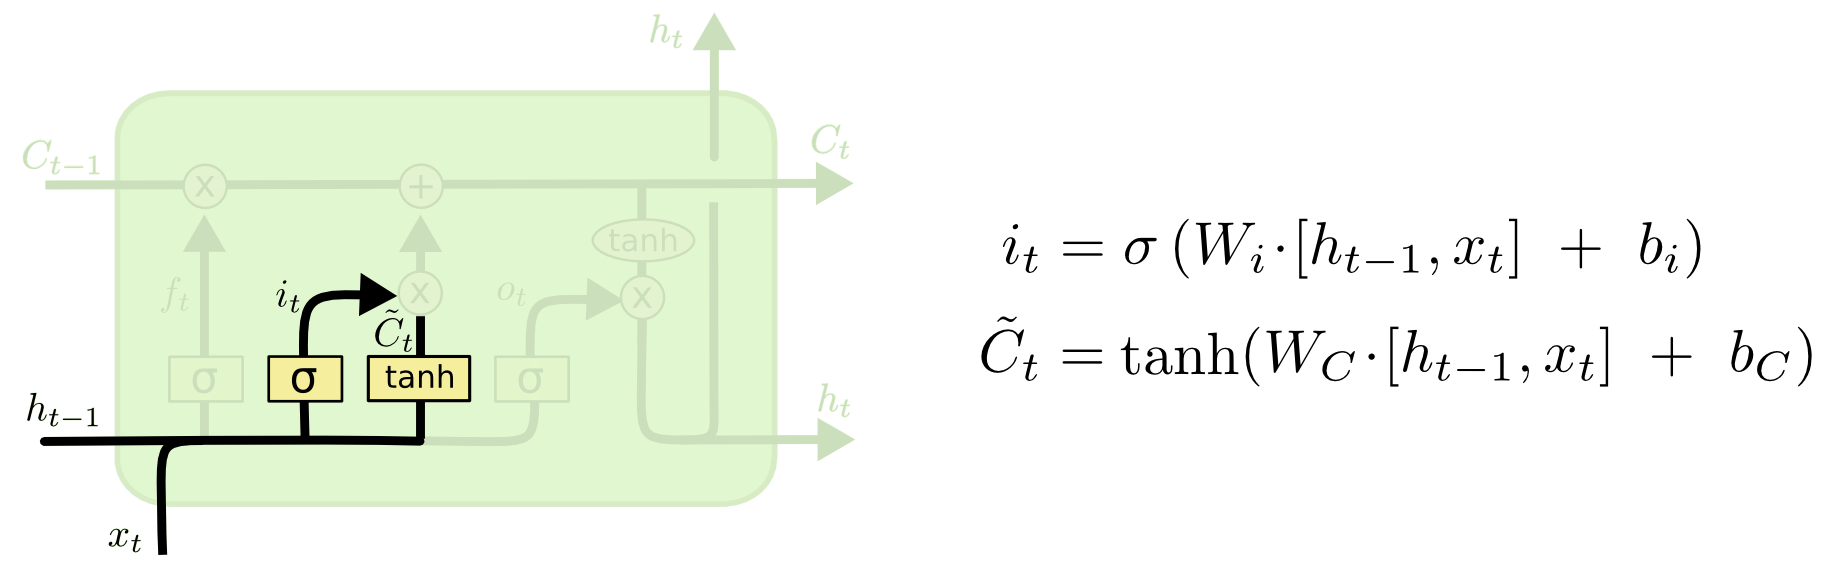
\includegraphics[width=0.8\linewidth]{../Report/imgs/lstm_explanation_step2}}
		\end{figure}
		
		\begin{figure}[h]
			\center{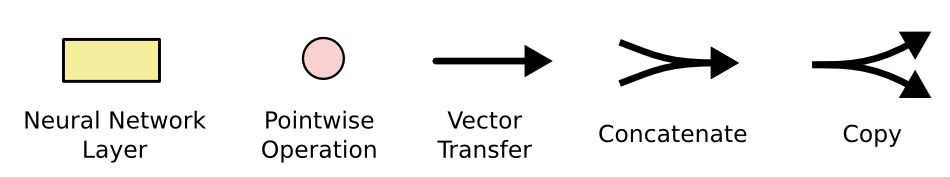
\includegraphics[width=0.6\linewidth]{../Report/imgs/lstm_operations}}
		\end{figure}
		
	\end{frame}

	\begin{frame}
		\frametitle{Объясняя LSTM (часть 3)}
		
		\begin{figure}[h]
			\center{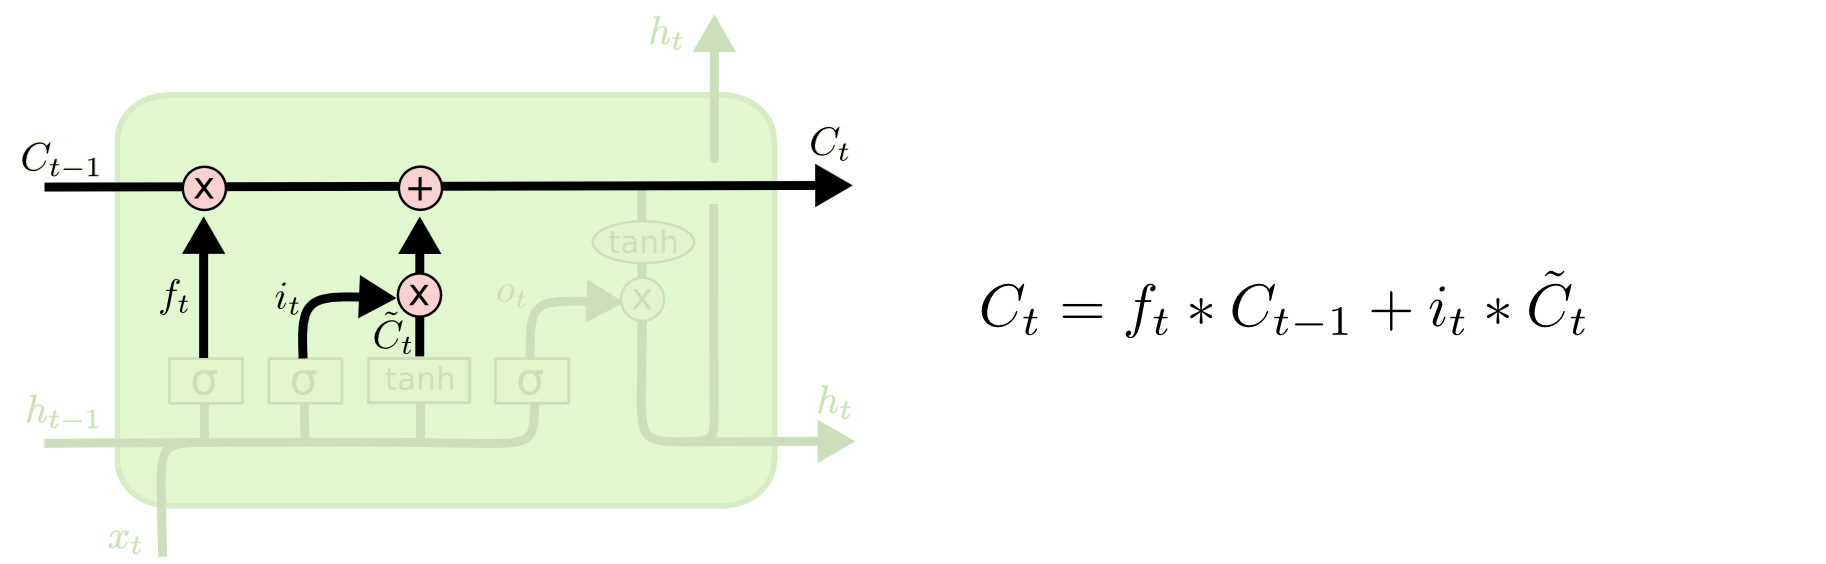
\includegraphics[width=0.8\linewidth]{../Report/imgs/lstm_explanation_step3}}
		\end{figure}
	
		\begin{figure}[h]
			\center{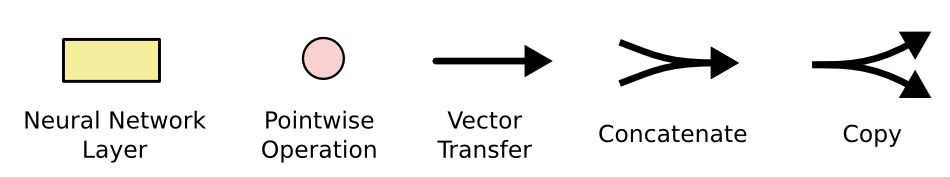
\includegraphics[width=0.6\linewidth]{../Report/imgs/lstm_operations}}
		\end{figure}
		
	\end{frame}

	\begin{frame}
		\frametitle{Объясняя LSTM (часть 4)}
		
		\begin{figure}[h]
			\center{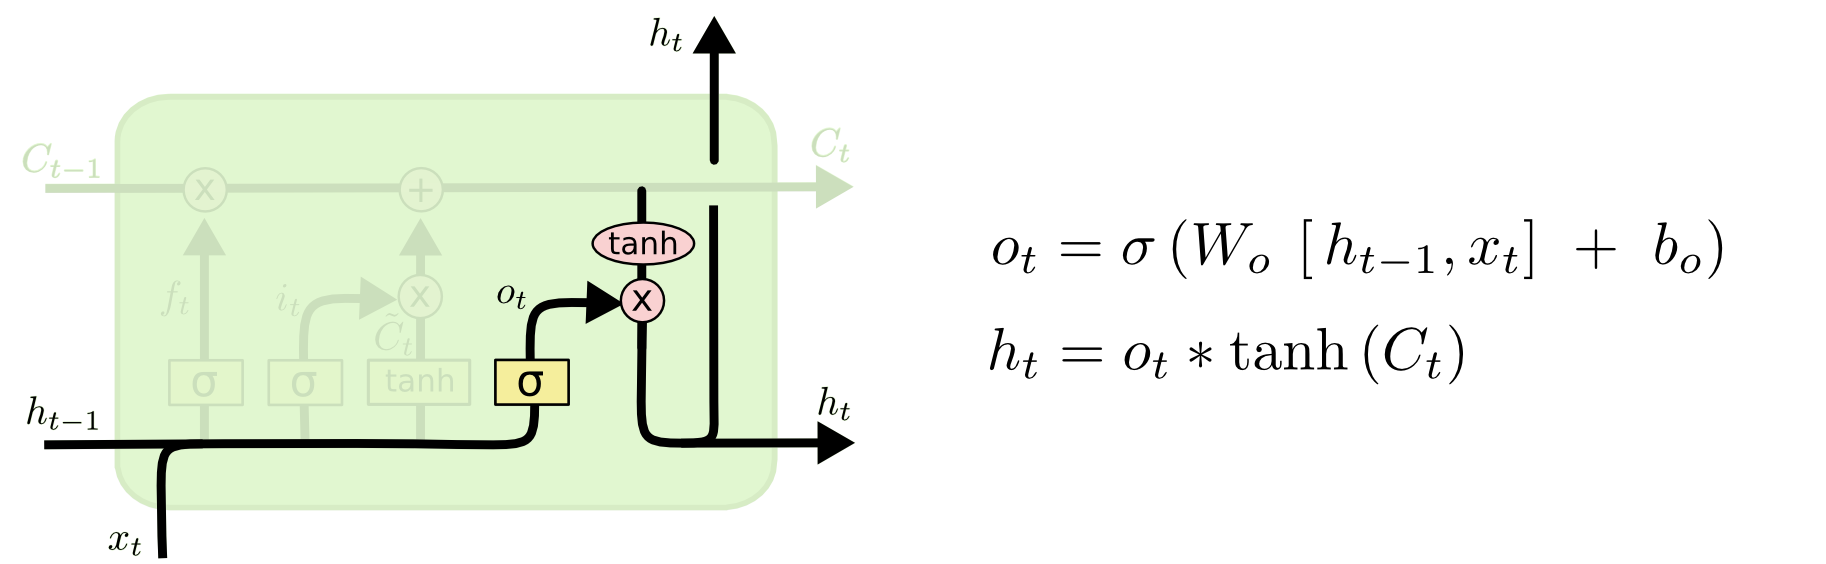
\includegraphics[width=0.8\linewidth]{../Report/imgs/lstm_explanation_step4}}
		\end{figure}
		
		\begin{figure}[h]
			\center{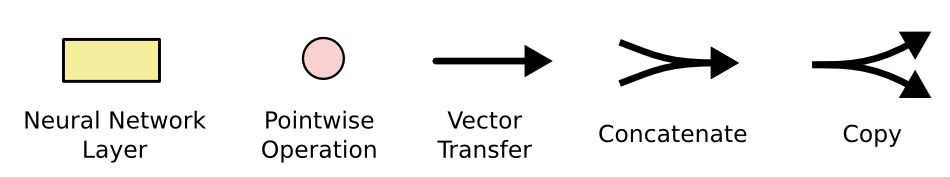
\includegraphics[width=0.6\linewidth]{../Report/imgs/lstm_operations}}
		\end{figure}
		
	\end{frame}
	
	\begin{frame}
		\frametitle{Модификации LSTM}
		LSTM с <<замочными скважинами>> (peepholes)
		
		\begin{figure}[h]
			\center{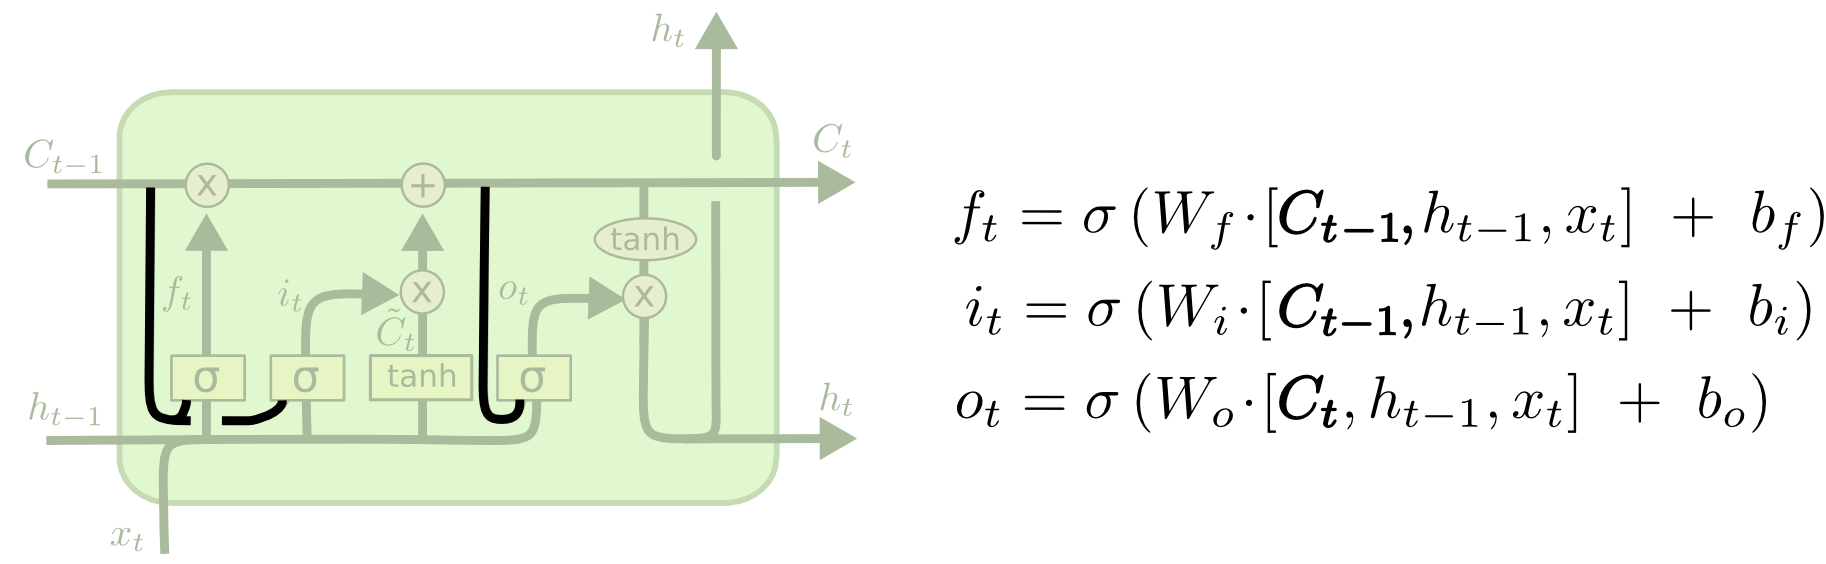
\includegraphics[width=0.8\linewidth]{../Report/imgs/lstm_peepholes}}
		\end{figure}
	
		Все фильтры <<подглядывают>> вектор состояния $C_{t-1}$ или $C_t$.
		
		\medskip
		
		Увеличивается число параметров модели.
		
		\medskip
		
		Замочную скважину можно использовать не для всех фильтров.
		
	\end{frame}
	
	\begin{frame}
		\frametitle{Модификации LSTM}
		LSTM Gated recurrent units (GRU)
		
		\begin{figure}[h]
			\center{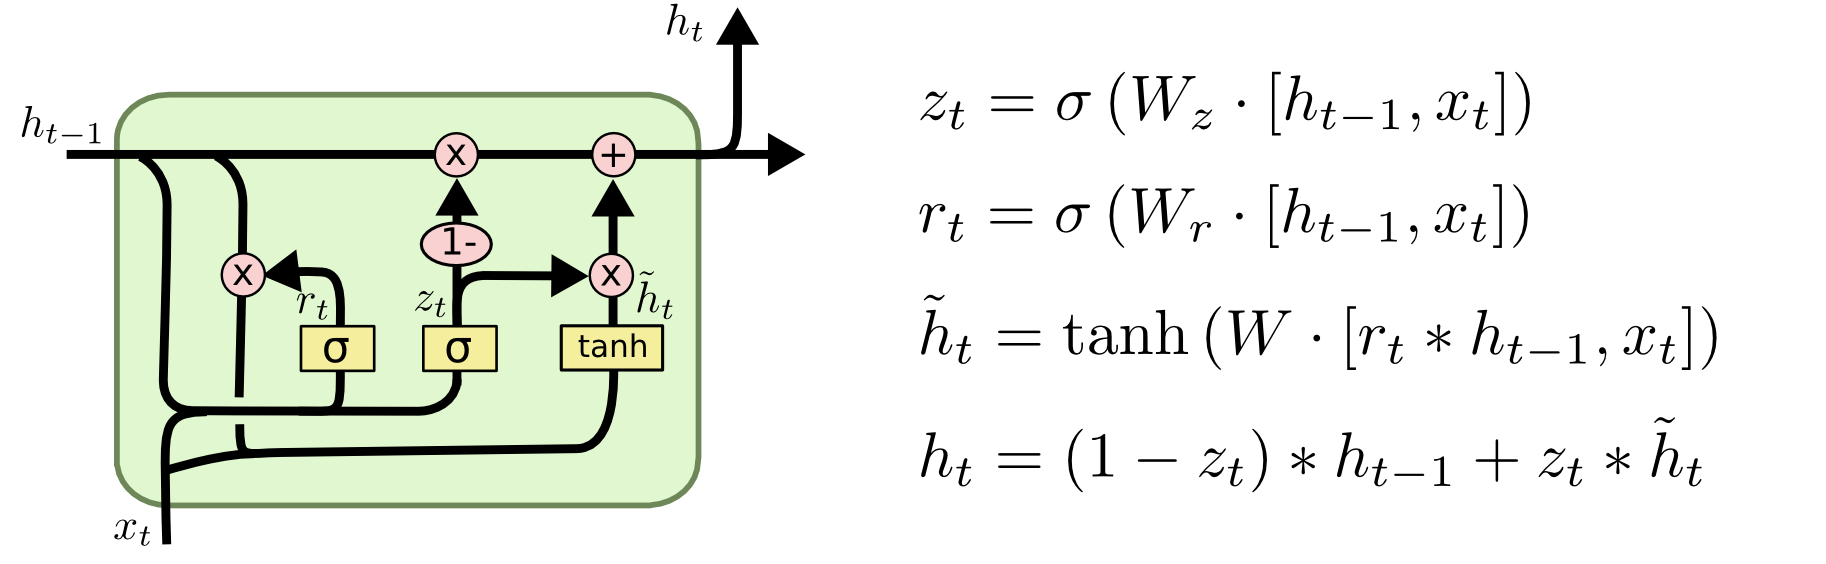
\includegraphics[width=0.8\linewidth]{../Report/imgs/lstm_gru}}
		\end{figure}
		
		Используется только состояние $h_t$, вектор $C_t$ не вводится.
		
		\medskip
		
		Фильтр обновления (update gate) вместо входного и забывающего.
		
		\medskip
		
		Фильтр перезагрузки (reset gate) решает, какую часть памяти нужно перенести дальше с прошлого шага.
		
	\end{frame}
	
	\begin{frame}
		\frametitle{Dropout}
	
		{\color{blue} Обучение:} обнуляем выход $h$-ого нейрона $\ell$-го слоя с вероятностью $p_\ell$.
		 
		$$a^{\ell+1}_{ih} = \xi^{\ell}_h f_h^{\ell}\big( \sum\limits_{j} w_{jh}a_{ij}^{\ell} \big), P(\xi^{\ell}_h = 0) = p_\ell$$
		
		{\color{blue} Применение:} вводим поправку
				 
			$$a^{\ell+1}_{ih} = (1 - p_{\ell}) f_h^{\ell}\big( \sum\limits_{j} w_{jh}a_{ij}^{\ell} \big)$$
			
		\begin{figure}[h]
			\center{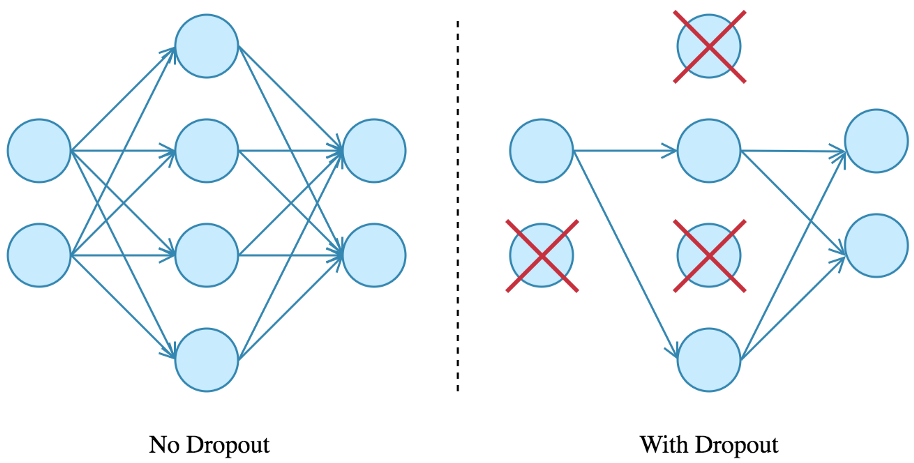
\includegraphics[width=0.5\linewidth]{../Report/imgs/dropout}}
		\end{figure}
		
	\end{frame}

	\begin{frame}
		\frametitle{Dropout}
		
		{\color{blue} Inverted Dropout:} $$a^{\ell+1}_{ih} = \dfrac{1}{(1 - p_{\ell})} \xi^{\ell}_h f_h^{\ell}\big( \sum\limits_{j} w_{jh}a_{ij}^{\ell} \big)$$
		
		\begin{itemize}
			\item регуляризация: из всех сетей выбираем  более устойчивую к утрате $pN$ нейронов.
			\item сокращаем переобучение, заставляя разные части сети решать одну и ту же исходную задачу. 
		\end{itemize}
		
	\end{frame}

	\begin{frame}
		\frametitle{Batch Normalization}
		
		$B = {x_i}$ --- пакеты (mini-batch) данных.
		Усреднение градиентов $\mathcal{C}(w)$ по пакету ускоряет сходимость.
		
		$B^{\ell} = \{u_i^{\ell}\}$ --- векторы объектов $x_i$ на выходе $\ell$-го слоя.
		
		{\color{blue} Batch Normalization:}
		
		\begin{enumerate}
			\item Нормировать каждую $j$-ю компоненту вектора $u_i^{\ell}$ по пакету:
			
			$$ \hat{u}_{ij}^{\ell} = \dfrac{u_{ij}^{\ell} - \mu_j}{\sqrt{\sigma^2_j + \varepsilon}}; \; \; \;
			 	\nu_j = \dfrac{1}{|B|} \sum\limits_{x_i \in B} u_{ij}^{\ell}; \; \; \;
			 	\sigma^2_j = \dfrac{1}{|B|} \sum\limits_{x_i \in B} (u_{ij}^{\ell} - \nu_j)^2. $$
			\item Добавить линейный слой с настраиваемыми весами:
				$$ \tilde{u}_{ij}^{\ell} = \gamma_j^\ell \hat{u}_{ij}^{\ell} + \beta_j^\ell $$
			\item Параметры $\gamma_j^\ell$ и $\beta_j^\ell$ настраиваются с помощью back-propagation.
		\end{enumerate}
		
		
	\end{frame}
	
\end{document}